\chapter{Introduction}\label{ch:Introduction}
{\bf Abstract}\hspace{0.2cm} In this chapter.


\lettrine[lines=2]{\color{darkocre}Q}{uantum physics} methods play an
increasingly important role in many
domains of science. Modern mathematical tools are numerous and require
serious effort to master. The algebra and calculus of \emph{tensors}
are good examples of this.

The goal of this book is to explain tensors by
showing them in action and in relation to less complicated
mathematical objects, such as vectors and numbers. Understanding
numbers and vectors is
essential for understanding tensors, therefore the former two are
discussed in details.

The development of concepts will happen the following direction:
\begin{align*}
\textrm{Numbers}\quad\rightarrow\quad\textrm{Vectors}\quad\rightarrow\quad\textrm{Tensors.}
\end{align*}
We will start with reviewing numbers as the simplest mathematical
objects, and will consider operations on numbers -- functions -- in a
general and more abstract way than one usually does in school. Many
abstract concepts related to numbers and functions will be useful for
studying vectors and tensors.

From numbers and numeric functions we will move on to vectors. Vectors
are closely connected to numbers and can't even be properly defined
without the latter. Vectors\index{Vector} are more powerful
than numbers and represent the next step in the hierarchy of
mathematical objects. Vectors and functions on vectors (operations or
operators\index{Operator}) provide many new concepts that are crucial for
understanding of tensors.

Careful study of vectors and functions on vector (operators)
will inevitably lead us to tensors. Tensors and vectors are as
intimately related, as vectors and numbers. In fact, having studied
the basics of tensor algebra, we will see that numbers, vectors, and
tensors are conceptually connected. We will be able to recognize that
numbers are\footnote{In a certain sense which will become clear
after reading the book.} very reduced tensors; numbers are tensors of
 rank zero. In a similar sense, vectors are not completely reduced
 tensor; vectors
are tensors of rank one. Therefore, the progression of the topics from
numbers to tensors can be viewed as follows:
\begin{align*}
  & \textrm{Numbers} \quad & \rightarrow \quad & \textrm{Vectors} \quad &
  \rightarrow \quad & \textrm{Tensors.}\\
  & \textrm{Tensors}^{(0)} \quad & \rightarrow  \quad & \textrm{Tensors}^{(1)}
  \quad & \rightarrow \quad & \textrm{Tensors}^{(2+)}\,.
\end{align*}
Here the superscript in parentheses indicates the rank of the
tensor\footnote{Don't worry if the concept of \emph{rank} seems
unclear right now -- it will be explained in due time.}.


As we move from numbers to tensors, the level of abstraction\index{Abstraction}
increases. To a significant degree, the difficulty of understanding
tensors is due to high level of abstraction used in the definition
of tensors as mathematical objects. Abstraction is the price we pay
for more powerful and versatile tools. But more powerful tools are
needed as scientists address more and more advanced problems.

The inventions of numbers, algebra, and then calculus were monumental
breakthroughs. The transition from numbers to vectors and then to
tensors is a more natural process that occurred rather quickly on
the scale of the history of science.


 \section{Who Needs Tensors?}
Although physicists make heavy use of tensors, today thousands of
scientists -- not only physicists -- use
the mathematical methods of tensors. Tensor mathematics (the algebra
and calculus of tensors) is a \emph{tool}; it is a fitting tool for
some problems, and not too fitting for others. This
situation is quite analogous to \emph{vector algebra and calculus}.


Tensor literacy will enrich you and will open doors to new
problems and new methods of their analysis. The following historical
episode illustrates the point well.

In October of 1912, Albert Einstein\index{Einstein} wrote in a letter to his physicist
friend Arnold Sommerfeld:
\begin{mybio}{Einstein on General Relativity}
  I am now exclusively occupied with the problem of gravitation theory
and hope, with the help of a local mathematician friend, to overcome
all the difficulties. One thing is certain, however, that never in my
life have I been quite so tormented. A great respect for mathematics
has been instilled within me, the subtler aspects of which, in my stupidity,
I regarded until now as a pure luxury. Against this problem [of
  gravitation] the original problem of the theory of relativity is
child’s play.
\end{mybio}
In the period from 1905 to 1916 Einstein was feverishly working on the
General Theory of Relativity\index{General relativity} -- the next
best theory of gravity since
Newton. The mathematics of general relativity is based on the calculus
of tensors, created by Italian mathematicians Ricci-Curbastro and
Levi-Civita roughly a decade before Einstein started working on the
problem of gravity.

To overcome the mathematical difficulties, Einstein used the help of
his friend and former classmate Marcel Grossmann\index{Grossmann Marcel}, who was an
expert in tensor calculus and non-Euclidean geometry. The general
theory of relativity was the first physical theory to use the power of
tensors (in combination with profound physical insights) to achieve
remarkable breakthrough. Since then, the
methods of tensor calculus and non-Euclidean geometries have been used
in many physical theories and problems.

In the end of the book (Section \ref{sec:tensorsComputation} on page
\pageref{sec:tensorsComputation}) a less dramatic example is
given. The example describes a real-world situation when the
understanding of vectors and tensors lead to significant practical
benefits.

\section{Naive Notion of Tensors}\label{sec:TensorNaive}
We may think of tensors as some kind of ``super-numbers.'' In what
sense tensors are numbers and what makes them ``super?''

Similar to numbers, tensors can be added and subtracted. Also, tensors
can be ``scaled'' by multiplying them by ``normal'' numbers, like $2$
or $\pi$.

Unlike numbers, tensors support richer set of operations. Given two
tensors, we can ``kind-of-multiply'' them to get either a simple
number as the result (\emph{scalar product}, see Section
\ref{sec:Dol}), or we can get another
tensor, somewhat ``bigger'' than the original two (\emph{tensor
product}, see Section \ref{sec:TensorProduct}.)

Looking at the evolution of the concept of number, we can
see the series of steps to higher levels of \emph{generality},
\emph{efficiency} , and
\emph{abstraction}\index{Abstraction}: From natural numbers, to whole numbers, to
fractions, to real and then to complex numbers. At each step new
\emph{mathematical objects}\index{Mathematical!object} are introduced that can be added and
multiplied in a ``usual way.''

Tensors come as the result of quite natural evolution of
``number-like mathematical objects.'' Tensors extend the notion of
numbers, all the way through vectors into a new and very powerful
realm. If numbers are ``bare quantities,'' and vectors are
``quantities with direction'' (e.g., velocity in physics), then
tensors are ``quantities with shape.''

Tensors are naturally and closely connected with numbers and
vectors. In fact, numbers and vectors \emph{are tensors!}

\begin{mybio}{Tensors Naively Defined}
Tensors are \emph{mathematical objects} that cover and extend the
concepts of numbers and vectors. As more powerful mathematical
objects, tensors support many algebraic operations, including
addition, subtraction, and scaling by a number.

Tensors might be viewed as ``quantities with shape,'' in
analogy with vectors -- ``quantities with direction.''

Numbers and vectors represent the lowest ``tiers'' (called
\emph{ranks}) in the hierarchy of tensors.

Finally, tensors generalize the idea of \emph{linear functions} (see
subsection \ref{subsec:linearFunctions} on page
\pageref{subsec:linearFunctions} and also Section
\ref{sec:LinearOperators}). Tensors of higher ranks can ``act'' on
tensors of lower ranks in a very simple way, resembling familiar
multiplication.
\end{mybio}

\section{Example Definitions}\label{sec:ExampleDefinitions}
Now what are tensors more rigorously? Can we give a short definition
to this concept?
Let us take a look at several examples and see whether they shed
sufficient light. The definitions given below differ from each other,
but they simply convey \emph{the same idea in different ways}.

The Encyclopedia of Mathematics
\footnote{\url{https://encyclopediaofmath.org/wiki/Tensor_on_a_vector_space}}
provides the following definition:

%\begin{tcolorbox}[colback=white!85!ocre, title=Tensors Definition 1]
\begin{mydef}{Tensors Definition 1}\\
  \small
Tensor\index{Tensor} on a vector space $V$ over a field $k$ is an element $t$ of the
vector space
\begin{equation*}
	T^{p,q} (V) = (\otimes^p V)\otimes (\otimes^q V^*)\,,
\end{equation*}
where $V^*=\textrm{Hom}(V, k)$ is the dual space of $V$.
\label{tcb:tensorDefinition1}
\end{mydef}
%\end{tcolorbox}
To understand this defintion we first need to understand what
\emph{vector space}\index{Vector!space} is, what \emph{field} is, what \emph{dual} means,
and what is going on with superscripts and circles (e.g., in
$\otimes^q$).


Wolfram Math World\footnote{\url{https://mathworld.wolfram.com/Tensor.html}}
provides another view of tensors:
%\begin{tcolorbox}[colback=white!85!ocre, title=Tensors Definition 2]
\begin{mydef}{Tensors Definition 2}\\
  \small
An $n$th-rank tensor\index{Tensor} in $m$-dimensional space is a mathematical object
that has $n$ indices and $m^n$ components and obeys certain
transformation rules.
\end{mydef}
%\end{tcolorbox}
Here we encounter new concepts, such as: \emph{rank of a tensor},
$m$-\emph{dimensional space}, \emph{indices}, \emph{components}, and
some kind of \emph{transformation rules}. They all will be discussed
later in the book.

Yet another definition can be found in the book \emph{Encyclopedia Of
Mathematics}\footnote{\emph{Encyclopedia Of Mathematics}, James
Tanton, Facts On File, Inc, 2005}

%\begin{tcolorbox}[colback=white!85!ocre, title=Tensors Definition 3]
\begin{mydef}{Tensors Definition 3}\\
  \small
Just as a \emph{vector} is a mathematical quantity
that describes translations in two- or three-dimensional
space, a tensor is a mathematical quantity used to
describe general transformations in $n$-dimensional
space. Precisely, if the locations of points in $n$-dimensional
space are given in one coordinate system\index{Coordinate!system} by
$(x^1,x^2,…,x^n)$ and in a transformed coordinate system
by $(y^1, y^2,…,y^n)$ (it is convenient to use superscripts
rather than subscripts), then a “rank 1 contravariant
tensor” is a quantity $T$, with single components, that
transforms according to the rule:
\begin{equation*}
	T^i_{new} = \sum\limits_{r=1}^{n} \frac{\partial y^i}{\partial x^r} T^r\,.
\end{equation*}
\end{mydef}
%\end{tcolorbox}
Again we face a wall of new concepts: \emph{vectors},
\emph{transformations}, $n$-\emph{dimensional space},
\emph{contravariant tensors} and their \emph{components}. Without
clear understanding of these concepts, it is impossible to learn what
tensors are.


The definitions given above are typical. They provide a good way to \emph{end}
the study of tensors, to summarize everything learned about
them. However, they are not good starting points. It is better to
arrive at the concept of tensor gradually, going from numbers, through
vectors, to tensors. This path starts in the next chapters. But before we
 begin, a couple of preliminary remarks are needed.

\section{Diagrams}
Sometimes to illustrate mathematical concepts and \emph{relations between them}\index{Relations},
we will use diagrams. Diagrams are helpful in highlighting
some general features of \emph{mathematical structures}\index{Mathematical!structure}.

Let us study an example, shown in the Figure \ref{fig:diagrams}. A
collection of cars in a parking lot -- Figure \ref{fig:diagrams}(a) --
can be schematically represented
as a set of \emph{points} $\Lambda$ -- Figure
\ref{fig:diagrams}(b). Each point of the set $\Lambda$ corresponds to a
certain car in the parking lot. Apart from the set of cars $\Lambda$, the Figure
\ref{fig:diagrams}(b) contains other sets, denoted as $K$, $N$, and
$B$. These sets correspond to various values of cars' properties, such
as color (set $K$), mileage (set $N$), and so on. The set $B$ is a very
important set --
called \emph{Boolean set}\index{Set!Boolean}. Boolean set has just two points, one
labeled $t$ for True, the other labeled $f$ for False.

Reduced to a point of the set $\Lambda$, a car looses its individuality
and those parameters that
make it unique (make, color, milage, etc.) This is remedied by using
other sets, such as the set of
various colors $K$ or the set $N$ of numbers that can represent
mileage, and so on.
\begin{figure}[htbp]
  \centering
  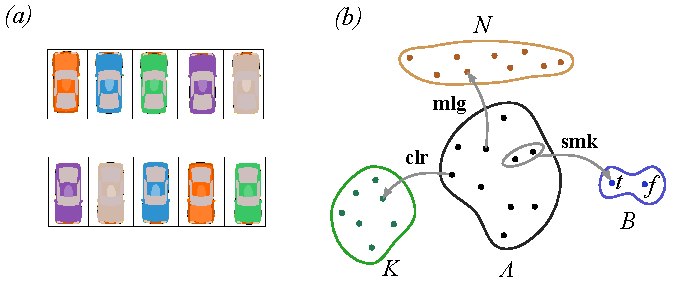
\includegraphics[scale=1.0]{../01Introduction/pics/diagrams}
  \caption{Diagrams are used to graphically represent sets of objects
    and relationships between them. Arrows can connect (map) elements
    of one set with another. Such mappings may have names: {\bf mlg}
    returns mileage for a given car, {\bf clr} -- color, and {\bf smk}
  determines whether two cars are of the same make.}
  \label{fig:diagrams}
\end{figure}

A particular property of a car-point
can then be represented using an arrow that connects the car-point to
another point in the relevant set. We say that such an arrow \emph{maps}\index{Map}
points of one set into another set. The Figure\ref{fig:diagrams}(b)
shows three maps: $\textrm{\bf mlg}$ gives the mileage for each car from the
set $\Lambda$, $\textrm{\bf clr}$ gives the color for each car, and
$\textrm{\bf smk}$ compares whether two cars have the same make.

%\begin{tcolorbox}[colback=white!85!ocre, title=Problem]
\begin{exercise}
Extend the diagram from the Figure \ref{fig:diagrams}(b), adding a set
of different car makes (e.g., Ford, Toyota, Fiat, etc.) Come up with a
mapping from this set into the Boolean set $B$.
\label{exe:carMakesSet}
\end{exercise}
%\end{tcolorbox}

\section{Schematics}
To illustrate the concepts of functions, operators, their structures and
properties, we will be using schematics\index{Schematic} like the one
shown in the Figure \ref{fig:schematicExample}.
\begin{SCfigure}%[htbp]
  %\centering
  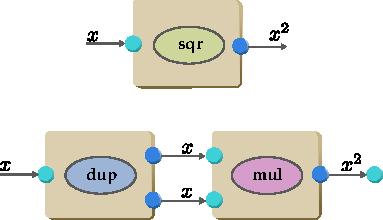
\includegraphics[scale=1.0]{../01Introduction/pics/schematicExample}
  \caption{Schematics can be used to represent functions, operators,
    their compositions and structure.}
  \label{fig:schematicExample}
\end{SCfigure}

A simple schematic element is represented as a box with inputs
and outputs. A box can have a name (label) which describes what the
function does to its input.  The number of inputs and
outputs can vary depending on the complexity of a function.

Various ``boxes'' can be combined (or \emph{composed}\index{Composition}) to create a
more complex structure. The Figure \ref{fig:schematicExample} shows
how the outputs of a function $\textrm{\bf dup}$ (duplicate its input) are
connected to the inputs of a function ($\textrm{\bf mul}$) that
multiplies its inputs. The result is a function that squares its input.

\section{Sets and Tuples}\label{sec:SetsTuples}
We will use many notational conventions in this book. Most of them
will be typical for mathematics: ``+'' denotes summation of two
quantities, ``='' means equality of two quantities, ``*'' -- a
multiplication, and parentheses in ``3*(x+y)'' are used to indicate
the order in which operations should be performed (first add and then
multiply).

At a certain point we will be discussing
``assemblies''\footnote{Collections, ensembles, groups, families --
these terms already have reserved specific mathematical meaning,
although they express similar idea.} of quantities. The simplest
example -- all natural numbers:
\[
1,\,2,\,3,\,4,\,5,\,\ldots, n,\,\ldots\,.
\]
We can also consider all letters of some alphabet:
\[
\textrm{a, b, c, d, e, f, g, h, i, j, k, l, m, n, o, p, q, r, s, t, u,
v, w, x, y, z}.
\]
Both these examples can be formally considered as \emph{sets}\index{Set} -- an
assembly of objects of similar kind. A set can given a special name
when it is referred to often. For example, the set of natural numbers
is denoted as
\[
\mathbb{N} = \lbrace 1,\,2,\,3,\,\ldots\rbrace\,.
\]
Note the use of curly braces -- they indicate that we are talking
about a set. Thus, for a set $\mathbb{S}$ with elements $a,\, b,\,
x$, and $y$ we write
\[
\mathbb{S} = \lbrace a,\, b,\, x,\, y\rbrace\,.
\]
The concept of a set is one of the most basic in mathematics and the
notation for sets is very standardized.

Another useful concept is called \emph{tuple}\index{Tuple}. A tuple is a
series of quantities that are related in a certain way, but can be of
different kinds. It is better to study examples:
\[
(3, \textrm{'a'})\quad\textrm{ -- couple },
\]
\[
(\vec{a}, \vec{b}, \theta)\quad\textrm{ -- triple },
\]
\[
(x, 4, \vec{a}, \sin)\quad\textrm{ -- quadruple }.
\]
A series of $n$ quantities is called $n$-tuple.

The most familiar use of tuples is the representation of coordinates
of points. In two dimensional plane:
\[
(x, y) = (2, 5)\quad\textrm{ -- couple (pair) }\,.
\]
In three dimensional space:
\[
(x, y, z) = (0, 1, -2)\quad\textrm{ -- triple }.
\]
Notice the difference between the coordinate tuples and the examples
given above: The tuples with coordinates contain only numbers, whereas
in the examples above, tuples contain quantities of various types. The
point is that tuples \emph{can} contain quantities of the same type,
but in general they do not. Another important difference between sets
and tuples is the importance of the order. Consider the set with two
elements:
\[
\mathbb{S} = \lbrace 0, 1\rbrace = \lbrace 1, 0\rbrace\,.
\]
The order in which we write the elements does not matter. In contrast,
the order is important for tuples:
\[
(0, 1) \ne (1, 0)\,.
\]
This inequality becomes obvious if we interpret these couples as
coordinates of points in a plane. The first pair correspond to the
point on the $x$ axis, while the second pair corresponds to the point
on the $y$ axis.

Finally, the tuples can be used to concisely describe
\emph{mathematical structures}\index{Mathematical!structure}. As a
simple example, consider the set
of whole numbers $\mathbb{Z}=\lbrace 0,\, \pm 1,\, \pm 2,\,\ldots \rbrace$.
  We can do many arithmetic operations with these numbers, but let us
focus only on the operation of addition. Then we can summarize our
interest using a triple as follows:
\[
(\mathbb{Z}, +, 0)\,.
\]
This expression says that we are studying a set of whole numbers $\mathbb{Z}$
equipped with a single operation ``$+$''. Moreover, we recognize that for
this operation there is a special element $0$ with ``neutral''
behavior:
\[
n + 0 = 0 + n = n
\]
for all numbers $n$ from the set $\mathbb{Z}$. We will encounter more
examples of this sort later in the book.

\vspace{1cm}
\section*{Chapter Highlights}
{\setstretch{1.5}\chhc
  \it
  \small
\begin{itemize}
\item Natural evolution of mathematical objects from numbers, through
  vectors, leads to tensors.
\item Each successive tier of mathematical object in the progression
  ``numbers, vectors, tensors''  is more abstract and more powerfull.
\item Numbers, vectors, and tensors are all conceptually connected.
\item Just like the use of vectors opens up new methods for solving
  abstract and applied problems, so the use of tensors opens up new,
  even more powerful, methods for solving problems in various domains
  of science.
\item Diagrams and schematics are helpful to illustrate various
  mathematical relations and structures.
\item Set is an assembly of objects of similar kind. It is one of the
  basic concepts in mathematics.
\item Tuple is an ordered sequence of elements related to each other
  by a common context. The elements of a tuple can be of different kind.
\end{itemize}
}
